%\documentclass[a4paper]{fhnwreport} %Legt grundlegende Formatierungen wie Schriftarten, Ort Seitenzahlen etc. fest.
%
%\graphicspath{{./graphics/}}%Change according to graphics folder!
%
%\begin{document}

\section{Software}
Die Anforderung des Auftraggebers beinhaltet, dass die Kommunikation zwischen Sensorplatine und Meldezentrale über die Powerline erfolgt und keine zusätzliche Leitung beanspruchen darf. Für die drahtlose Übertragung war die Idee die Kommunikation über ein kabelloses System, wie Bluetooth oder Wireless zu verwenden. Diese Idee wurde aufgrund der unbekannten Distanzen zwischen der Sensor- und Meldeplatine verworfen.Für diese Einkopplung wird ein fertiger Transceiver und ein Kommunikationsprotokoll verwendet. Die Kommunikation zwischen Mikrocontroller und Transceiver wird mit UART realisiert. Es wird auf der Sensorplatine ein Mikrocontroller ATMega328 verwendet.


\subsection{Sensorplatine}
Die Aufgabe der Sensorplatine besteht aus der Verarbeitung der gemessenen Daten und der Übermittlung der Daten. In der Abbildung \ref{fig:Software_Flussdiagramm_Sensorplatine} ist der Verlauf dieser Verarbeitung ersichtlich.

\begin{figure}[htbp] 
  \centering
     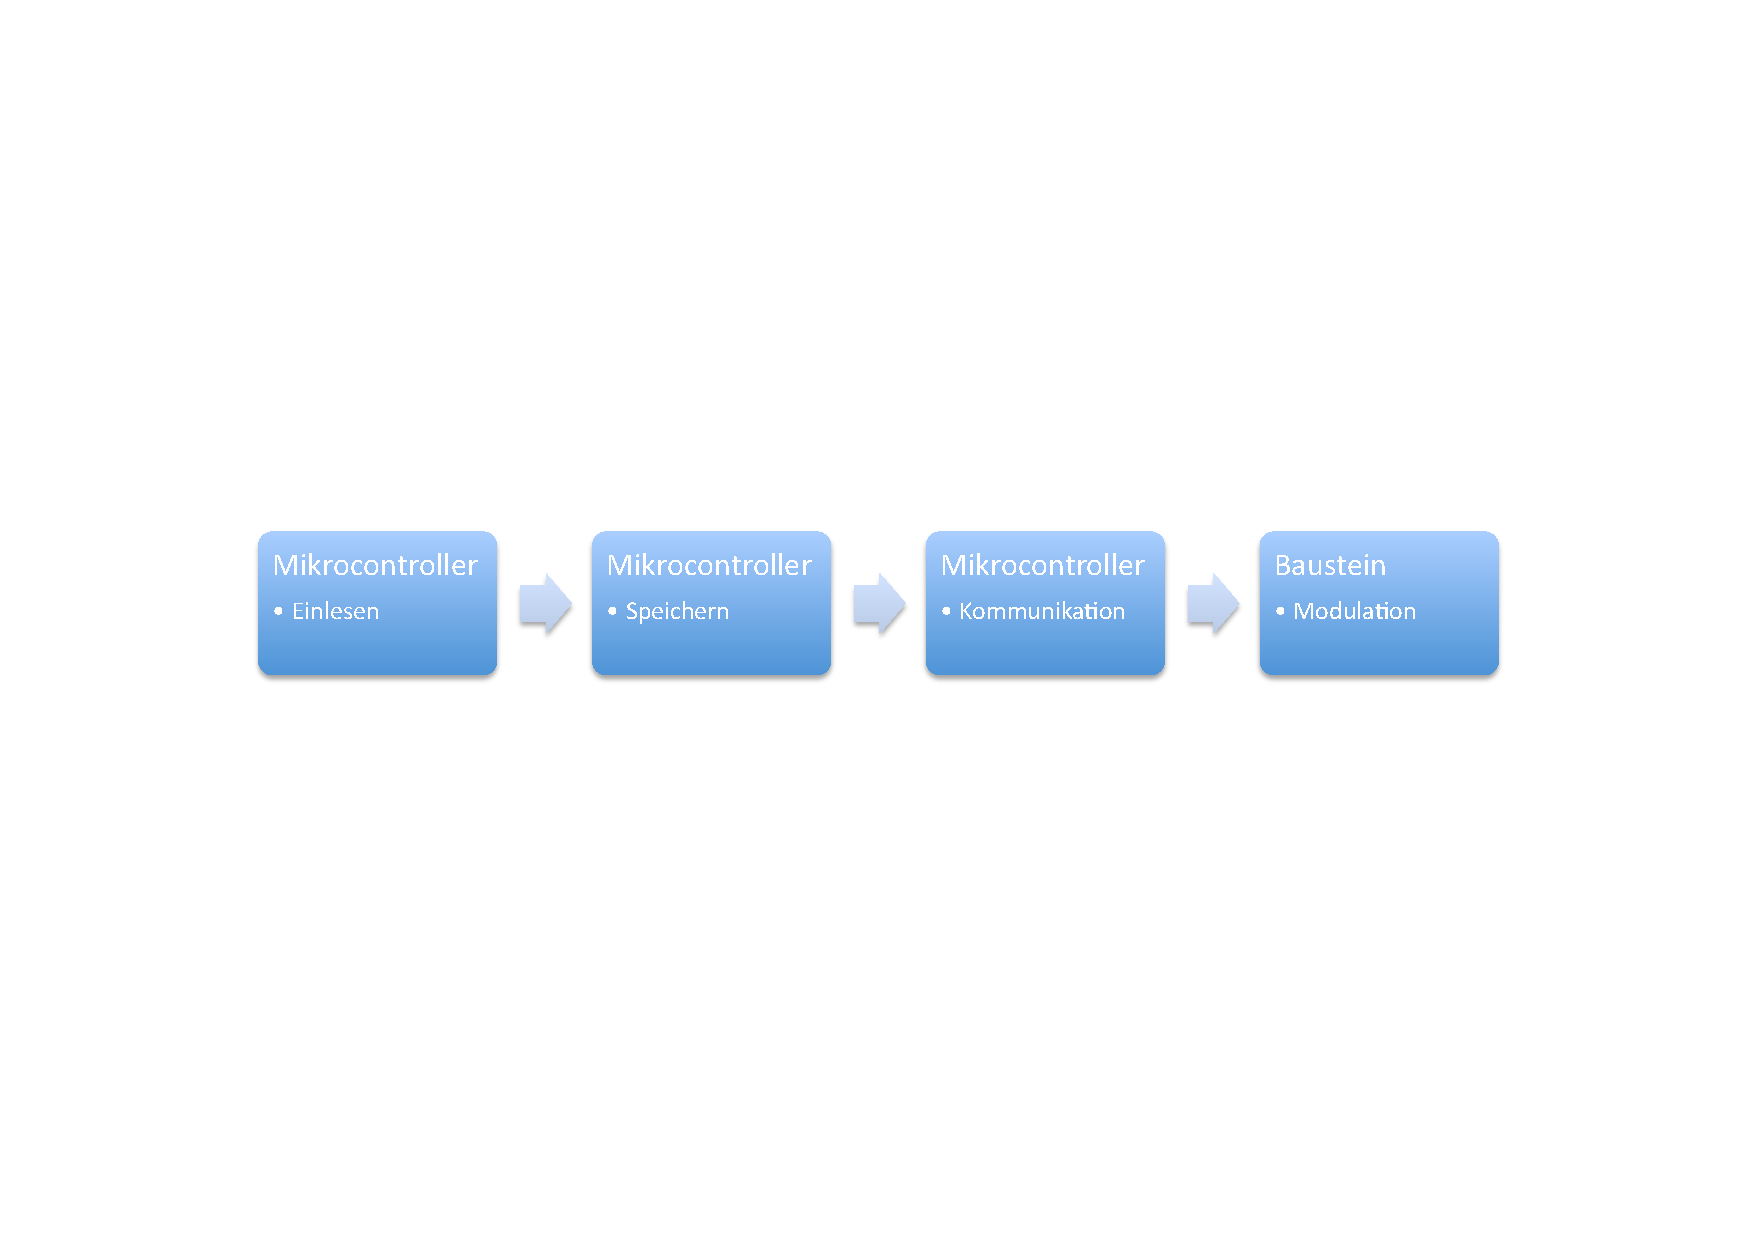
\includegraphics[width=1\textwidth]{graphics/Software_Flussdiagramm_Sensorplatine}
  \caption{Flussdiagramm Verlauf Programm Sensorplatine}
  \label{fig:Software_Flussdiagramm_Sensorplatine}
\end{figure}

Im ersten Schritt in der Abbildung \ref{fig:Software_Flussdiagramm_Sensorplatine} werden von der Messung die Daten eingelesen und in verwendbare Datentypen gespeichert. Die Kommunikation zum Transceiver wird über eine serielle asynchrone Schnittstelle stattfinden. Der Modulator wird die Messdaten auf die Leitung, Powerline Communication, induktiv einkoppeln. \\ Die Kommunikation soll unidirektional sein. Das Problem der Kollisionen soll wie folgt vermieden bzw. verringert werden: Innerhalb einer Stunde werden die Daten von allen Modulen mehrere Male gesendet, wobei die Verzögerung zwischen zwei Sendeversuchen eine statische und zufällige Teil enthält. Dies verringert die Wahrscheinlichkeit, dass zwei Kollisionen hintereinander auftreten.
Der Empfänger prüft die Vollständigkeit der Daten anhand einer Checksumme (CRC).

\subsection{Kontrollplatine}
Die Meldeplatine wird die Zentrale aller Sensorplatinen sein. Sie hat die Aufgabe den Betrieb der Anlage zu überwachen sowie die gesammelten und übermittelten Daten der Sensorplatinen auszuwerten. Für einen detektierten Fehler wird ein Relaiskontakt geschaltet und die fehlerhafte Stelle auf dem Display eingeblendet. Der gesamte Verlauf ist in Abbildung \ref{fig:Scheme_report_board} dargestellt.

\begin{figure}[h!] 
  \centering
     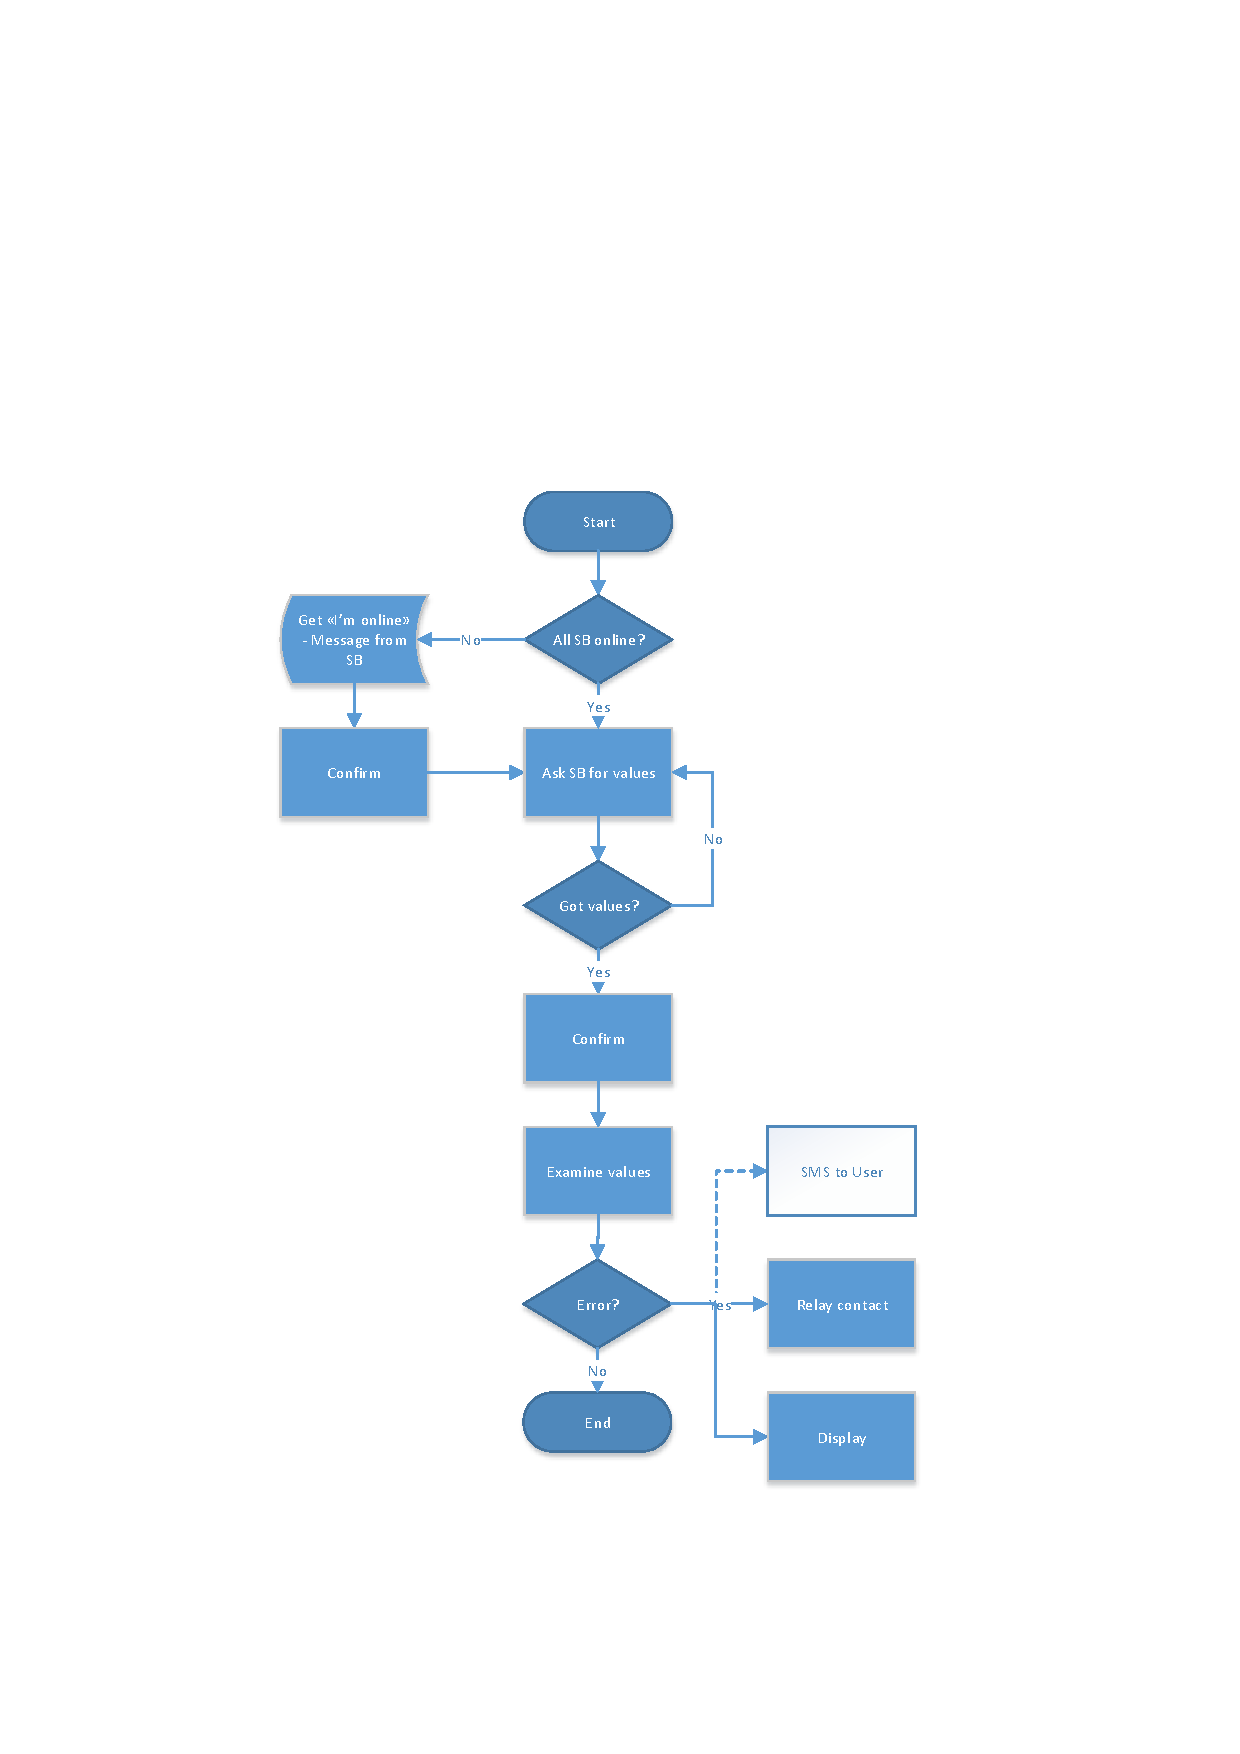
\includegraphics[width=0.5\textwidth]{graphics/Scheme_report_board}
  \caption{Flussdiagramm Verlauf Programm Meldeplatine}
  \label{fig:Scheme_report_board}
\end{figure}

\newpage

Damit die Meldeplatine die Anlage überwachen kann muss sichergestellt werden, dass alle Messwerte empfangen werden. Zu diesem Zweck erstellt die Meldeplatine bei der ersten Inbetriebnahme ein Register der Sensorplatinen (``Build register''). Danach beginnt sie die Messungen der Sensorplatinen zu empfangen (``Receive values'') und anschliessend auszuwerten (``Examine values''). Es besteht die Möglichkeit, dass eine Sensorplatine zur Zeit offline ist, fehlerhaft oder gleichzeitig mit einer anderen Sensorplatine Informationen sendet. Falls das der Fall sein sollte kommt es zu einer Warnung. Kommunizieren nach einer Wartezeit immernoch nicht alle Sensorplatinen richtig, kommt es zu einem Fehler, welcher einen Relaiskontakt betätigt und eine Meldung auf dem Display ausgibt.\\
Der Algorithmus für die Datenauswertung funktioniert nach dem arithemtischen Mittel. Es sagt aus, dass alle Datenpunkte addiert geteilt durch die Anzahl Datenpunkte einen Mittelwert ergibt. Weicht ein einzelner Datenpunkt stark vom Mittelwert ab, entspricht dieser einem Fehler. Um anschliessend das fehlerhafte Modul zu lokalisieren bekommt jede Sensorplatine eine Identifikationsnummer, die alle in einem Anlagenschema abgelegt sind.\\

Die Situation ``Nacht'' wird mittels dem Vergleich des Mittelwerts mit dem minimalen Spannungslevel (12V) ermittelt, sodass in dieser Zeit keine Fehler ausgegeben werden.




\subsection{Bedienung}
Die Meldeplatine besitzt ein Interface für Informationen über die Software und die Anlage. Über einige \todo{Anzahl Knoepfe definieren} Knöpfe kann das Menü gesteuert sowie Eingaben gemacht werden. Der Benutzer kann folgende Eingaben vornehmen: die Anlage benennen, die Menge der Photovoltaikmodule angeben und Meldungen quittieren. Desweiteren kann die aktuelle Spannung, aktuelle Leistung und die vergangenen Meldungen abgefragt werden. Die Spannung und Leistung der Anlage wird ausgegeben als das Mittel über die vergangenen 30 Tage, als aktuelles Max- und Minimum.
%\end{document}